
\chapter{Differentiated memory management controller for containers}

  The existing memory management controller posses a few issues when it comes to managing memory among containers in an
  over-committed scenario. We initially bring out these issues, and then propose a solution and evaluate our solution
  with respect to the existing controller.
  
  \section{Drawbacks of existing memory management for containers}
  \label{sec:controller_issues}
  
    We have used empirical evaluations to verify and demonstrate our hypotheses. These hypotheses bring out the issues existing container
    memory management controller---Memory \cg{}. We have used both a native cloud testbed and an derivative cloud testbed to establish 
    our issues.
    
    \subsection{Experimental setup}
    
      The following are the experimental setup configurations, metrics and workloads used to establish the correctness of our hypotheses
      in a native cloud environment.
      
       \subsubsection{Experimental configurations}
    
	The set of configurations used for an analysis of memory management techniques in a container environment must be relevant, 
	and easy to apply. The following configurations fit this criteria, and have been used for the evaluation.
	
	\begin{itemize}
	  \item \textbf{Number of containers:} The number of containers that are currently executing in the system.
	  \item \textbf{Memory soft limit of container:} The minimum promised memory to a given container by the system on which the 
    container is executing.
	  \item \textbf{Memory hard limit of container:} The maximum memory that can be assigned to a container by the system on which the 
    container is executing.
	  \item \textbf{Memory usage of each container:} The usage of a container at a given point in time, that is generated by the workload 
    executing inside the container.
	  \item \textbf{Workload:} The workload that is running inside each of the container. Workloads can vary based on the type of operation 
    they perform, the ratio of anonymous memory pages they consume to that of page cache pages.  
	  \item \textbf{External memory pressure:} The memory pressure that is generated in the system in order to reduce the free memory 
    available in the system and trigger memory reclamation. This pressure could be either generated by a process on the same system / driver 
    that is running in the host system.
	  \item \textbf{Size of machine:} Size of Machine refers to the maximum memory available in the system inside which all the 
    containers are executing.      
	\end{itemize}  
      
      \subsubsection{Metrics of interest}
      
	The following are the metrics of interest to us that would help us analyze the experiments.
	  
	    \begin{enumerate}
	    \item \textbf{Memory assigned to each container:} Total memory assigned to a container at any given instant
	    \item \textbf{Soft memory reclaimed for each container:} Memory reclaimed from each container using SMR
	    \item \textbf{Total memory reclaimed for each container:} Total Memory reclaimed from container (SMR + GLR)
	    \item \textbf{Memory reclaimed using GLR:} Memory reclaimed from all containers and other processes running on system using GLR
	    \item \textbf{Memory reassigned for each container:} Memory reassigned to each container on freeing up of memory
	    \item \textbf{Application specific metrics:} Application metrics of the workload running inside containers like throughput, total 
    time taken etc.
	    \end{enumerate}
      
      \subsubsection{Workloads}
      
	This section presents the list of workloads that we have used as primary candidates to evaluate our empirical evaluations. All 
    workloads are chosen keeping in mind the memory intensive nature of the requirement.  
	
	These are the list of Synthetic workloads we have used to establish our problem.
	  
	  \myparagraph{Stress}
	    Stress \cite{stress} is a deliberately simple workload generator for POSIX systems. It imposes a configurable amount of CPU, 
    memory, I/O, and disk stress on the system. It is written in C and has been developed by people at Harvard university. 
	  
	  \myparagraph{Memory hogger}
	    Memory Hogger is a simple C program that allocates an array of specified memory using a simple \texttt{malloc()} and repeatedly 
    writes to these array locations. This only consumes anonymous memory pages.
	  
	  \myparagraph{File hogger}
	    File Hogger is a simple python program that creates a file with specified size and repeatedly updates it line by line there by 
    consuming both anonymous pages and file backed pages.

	These are the list of real workloads we have used to show how the existing problems affect real work applications.
	  
	  \myparagraph{MongoDB}
	    MongoDB \cite{Mongodb} is an open-source, document database designed for ease of development and scaling. Classified as a NoSQL 
    database program, MongoDB avoids the traditional table-based relational database structure in favor of JSON-like documents with dynamic 
    schema. It follows a memory hungry approach where it tries to use up most of system and it actually leaves it up to the OS's VMM to tell it 
    to release the memory.

	\myparagraph{Redis}
	    Redis \cite{redis} is a in-memory data structure store, used as database, cache and message broker. It is used to store a large 
    number of in-memory key-value pairs. Its in-memory nature makes it a prime candidate to use it as a workload in our empirical evaluations.
      
	\myparagraph{YCSB benchmark}
	    We use YCSB \cite{cooper2010benchmarking} (Yahoo Cloud Server Benchmark) project as the benchmark to generate the clients evaluate 
    to the performance of our real workloads i.e MongoDB and Redis servers. The goal of YSCB is to develop performance comparisons of the new 
    generation of cloud data serving systems. It is a framework and common set of workloads for evaluating the performance of different 
    “key-value” stores.
    
  
    \subsection{Issues in native environment}
    
      We have tried to show the issues in container memory management using empirical analysis. We have taken our hypothesis/questions, 
      and mapped them to various experiments to illustrate the issues. Inferences were drawn based on the observations in the experiments. 
    
      \begin{figure}
	\centering
	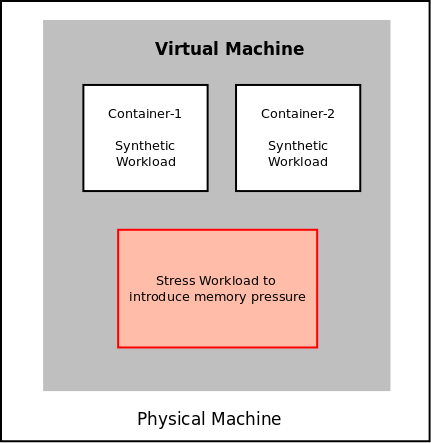
\includegraphics[width=0.5\textwidth]{images/controller_issues/native_testbed.png}
	\caption{Native container testbed}
	\label{img:native_setup}
      \end{figure}
      
       The native testbed consisted of running containers inside a host machine (running inside VM in our case) in complete isolation from 
the external environment as shown in Fig~\ref{img:derived_setup}. This setup which involved a native container testbed, was used to 
understand the existing memory reclamations and establish the problem in a native system using \textbf{synthetic workloads}.
	
      \subsubsection{Host}
	
	\begin{enumerate}
	  \item Intel Core i5-4430 processor @ 3.00GHz
	  \item 4 cores of CPU (with hyper threading support)
	  \item 1 TB of hard disk space
	  \item 8 GB RAM
	  \item Ubuntu 14.04 LTS desktop, 64 bit 
	  \item Kernel version 4.5
	  \item KVM Hypervisor
	\end{enumerate}
      
      \subsubsection{Guest}
	
	\begin{enumerate}
	  \item 3 cores of CPU (with hyper threading support)
	  \item 20 GB of virtual disk space
	  \item 2-6 GB RAM (based on experimental configuration)
	  \item Ubuntu 16.04 LTS desktop, 64 bit
	  \item Kernel version 4.7
	  \item Container technology: Docker
	\end{enumerate}
	
      Memory Hogger and File Hogger were used to generate the memory pressure inside the containers. External pressure was generated 
using Stress workload running directly on the host machine.
  
  
      The configuration in Table~\ref{table_native_base} is the base configuration for all experiments in this section. Any changes the base 
      configuration has been mentioned in the procedure of each of the experiment.

	\begin{table}	 
	  \begin{center}
	    \begin{tabular}{ l | c | c }
	      & Container-1 (M1) & Container-2 (M2) \\ 
	      \hline
	      \hline
	      Size of VM & \multicolumn{2}{c}{2 GB} \\	      
	      \hline
	      Workload & Memory Hogger & Memory Hogger \\
	      \hline
	      Hard Limit & 1000 MB & 1000 MB \\  
	      \hline
	      Soft Limit & 150 MB & 150 MB \\  
	      \hline
	      Memory Usage & 500 MB & 500 MB \\
	      \hline
	      Exceed & 350 MB & 350 MB \\
	      \hline 
	      External Pressure & \multicolumn{2}{l}{ 200 - 400 - 600 - 800 - 1000 MB} \\
	    \end{tabular}	    
	    \caption{Base configuration for native container experimentation}
	    \label{table_native_base}
	  \end{center}
	\end{table}
	
      Most experiments involved setting up of 2 containers. Workloads were used to introduce system memory pressure from containers. At 
      this point there was no memory pressure in the system (free memory was still available). Now the external pressure using Stress was 
      introduced after about 20s which created memory pressure in the system that triggered reclamation. The external pressure kept on increasing 
      by 200 MB in intervals of 40s. Each interval had a gap of 10s for memory to be reassigned to containers.
      
      \subsubsection{Reclamation above soft limits}
      
	\myparagraph{Hypothesis} 
	  Hypothesis to be verified,
	  \begin{enumerate}
	    \item Majority of reclamation when containers exceed occurs using SMR (Soft Memory Reclamation) 
	    \item SMR purely based on exceed value of the container
	    \item Containers that exceed equally are iteratively targeted
	  \end{enumerate} 
	  
	  \myparagraph{Procedure}
	    To demonstrate the correctness of our hypothesis we the base configuration described in Table~\ref{table_native_base} and change 
  the usage to 700 MB and soft limit to 350 MB there by simulating an scenario (Exp-1) where \textbf{Both containers exceeded by the same 
  values}.
	  
	  \begin{figure*}[t!]
	    \centering
	    \begin{subfigure}[t]{0.48\textwidth}
	      \centering
	      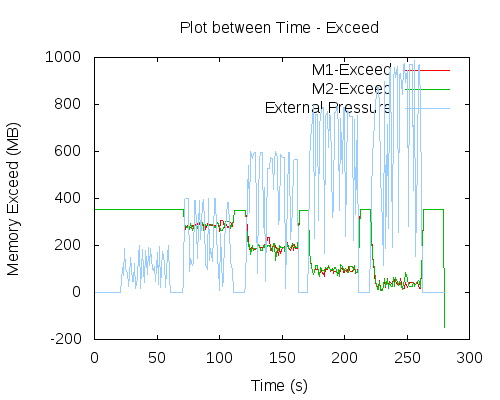
\includegraphics[width=1\textwidth]{images/controller_issues/exceed_only/Exceed.png}
	      \caption{Memory exceed plot}
	      \label{img_exceed_only_1_exceed}
	    \end{subfigure}
	    ~ 
	    \begin{subfigure}[t]{0.48\textwidth}
	      \centering
	      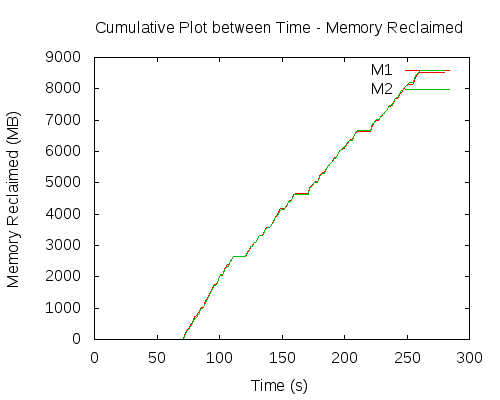
\includegraphics[width=1\textwidth]{images/controller_issues/exceed_only/Memory_Reclaimed.png}
	      \caption{Cumulative soft memory reclaimed plot}
	      \label{img_exceed_only_1_smr}
	    \end{subfigure}
	    ~ 
	    \begin{subfigure}[t]{0.48\textwidth}
	      \centering
	      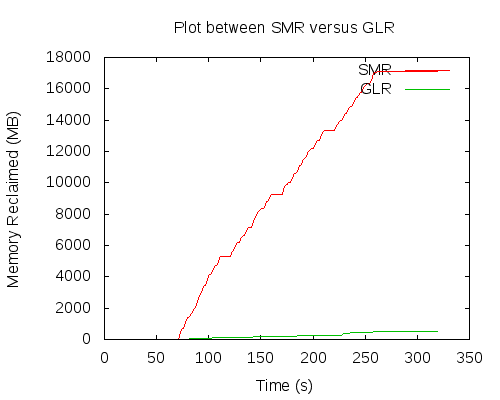
\includegraphics[width=1\textwidth]{images/controller_issues/exceed_only/compare.png}
	      \caption{SMR versus GLR}
	    \label{img_exceed_only_1_compare}
	    \end{subfigure}
	    \caption{Plots for analysis of reclamation when both containers are exceeding by same value}
	  \end{figure*}
	  
	  \myparagraph{Observations}
	    The following are the observations,
	    \begin{itemize}
	      \item As seen from Fig~\ref{img_exceed_only_1_exceed}, Fig~\ref{img_exceed_only_1_smr} - memory reclaimed from containers 
  iteratively from one after the other as their exceeds are same.
	      \item Fig~\ref{img_exceed_only_1_compare} shows how most reclamation when containers exceed occurs using SMR however it is seen 
  that there is minimum reclamation occurring using GLR as well.
	    \end{itemize}

	  \myparagraph{Inference}	
	    The following are the inferences,
	    \begin{itemize}
	      \item SMR is purely based on exceed value.
	      \item Most reclamation when containers exceed occurs using SMR, however the GLR kicks in every reclamation request to evict any 
  inactive page cache pages in the system (may/may not belong to container).
	      \item Containers that exceed equally are iteratively target for reclamation one after the other.
	    \end{itemize}
      
      \subsubsection{Reclamation below soft limits}
      
      \myparagraph{Hypothesis}
	Does our hypotheses of reclamation below soft limits falling back to native system reclamation hold good ?
	
      \myparagraph{Procedure}  
	To test the reclamation patterns in containers below soft limits, we created containers as mentioned in Table~\ref{table_native_base} 
  and changed soft limits (Exp-2) of both containers to 1000 MB there by making the current \textbf{usage of both containers below soft 
  limits}. We used hooks in the kernel code to track requests satisfied by soft memory reclamation (SMR) and global LRU based reclamation 
  (GLR).
	
	\begin{figure*}[t!]
	    \centering
	    \begin{subfigure}[t]{0.48\textwidth}
	      \centering
	      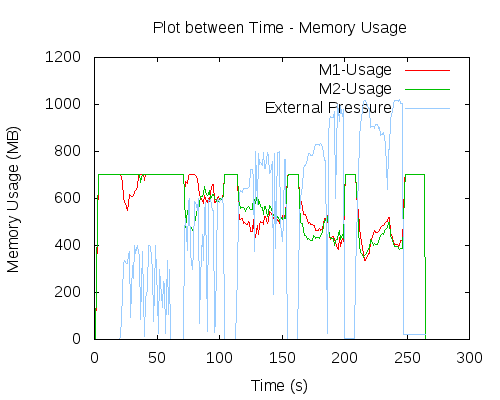
\includegraphics[width=1\textwidth]{images/controller_issues/global_lru/mu.png}
	      \caption{Memory Usage Plot}
	      \label{img_no_sl_mu}
	    \end{subfigure}
	    ~ 
	    \begin{subfigure}[t]{0.48\textwidth}
	      \centering
	      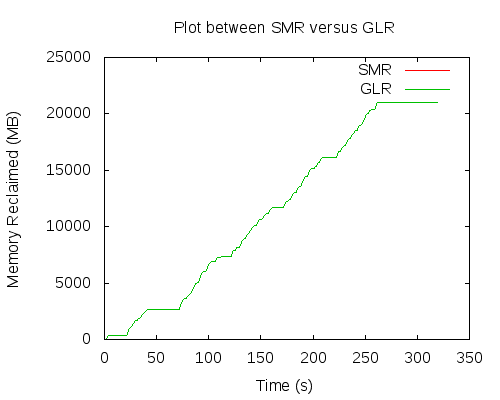
\includegraphics[width=1\textwidth]{images/controller_issues/global_lru/compare.png}
	      \caption{SMR versus GLR Plot}
	      \label{img_no_sl_global_vs_local}
	    \end{subfigure}
	    \caption{Plots for when both containers are having same usage but no exceeds}
	  \end{figure*}
	
	\myparagraph{Observations}
	  The following are the observations.
	  \begin{itemize}
	    \item As seen from Fig~\ref{img_no_sl_mu}, there is no hand-in-hand reclamation that occurs to containers below their soft 
  limits although the containers are running the same workload, unlike hand in hand reclamation that occurs in memory usage above soft limits.
	    \item Since both containers are below SL, all reclamation is occurring using the GLR (Global LRU based reclamation) as seen by 
  Fig~\ref{img_no_sl_global_vs_local}
	  \end{itemize}

	\myparagraph{Inferences}
	  The following are the inferences.
	  \begin{itemize}
	    \item Containers with memory usage below soft limits reclamation falls back to native system GLR.
	    \item Reclamation using GLR is haphazard and there is no control over it. 
	  \end{itemize}
   
     \subsubsection{Effect of workloads characteristics on reclamation}
      
	\myparagraph{Question}
	Questions of our interest,
	    \begin{enumerate}
	      \item Effect of workload characteristics on reclamation
	      \item How much of memory is reclaimed from a container in a single reclamation SMR request ?
	    \end{enumerate}
	  
	  \myparagraph{Procedure}
	    We took our base configuration as described in Table~\ref{table_native_base}. However we ran two workloads in this case - Memory 
  Hogger (Exp-4a) and File Hogger (Exp-4b) workloads on it as native theory suggests that containers with page cache pages might be 
  victimized at larger the way it occurs with GLR.	
	  

	  \begin{figure*}[t!]
	    \centering
	    \begin{subfigure}[t]{0.48\textwidth}
	      \centering
	      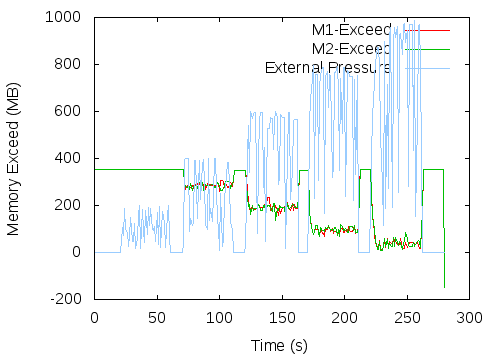
\includegraphics[width=1\textwidth]{images/controller_issues/workload/1/Exceed.png}
	      \caption{Exceed plot for memory hogger}
	      \label{img:workload_1_exceed}
	    \end{subfigure}
	    ~ 
	    \begin{subfigure}[t]{0.48\textwidth}
	      \centering
	      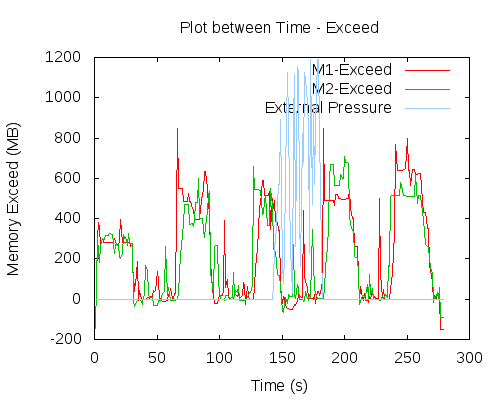
\includegraphics[width=1\textwidth]{images/controller_issues/workload/2/Exceed.png}
	      \caption{Exceed plot for file hogger}
	      \label{img:workload_2_exceed}
	    \end{subfigure}
	    \caption{Plots for analyzing effect of workloads characteristics on reclamation}
	  \end{figure*}		
	    
	  \myparagraph{Observations}
	  The following were the observations,	  
	  \begin{itemize}
	    \item The exceed goes hand in hand as expected but with larger deviation in Fig~\ref{img:workload_1_exceed} and 
  Fig~\ref{img:workload_2_exceed}
	    \item The larger deviation can be accounted to larger reclamation chunks in workloads that have page cache pages similar to how 
  reclamation targets page cache pages in native system
	    \item Further empirical analysis of the reclamation chucks gave us the reclamation chucks to be 
		\begin{center}
		    Reclamation chuck = Anonymous memory pages (\textless 25MB) + Page cache pages
		\end{center}
		In both cases pages from inactive zones were reclaimed before trying to reclaim from active lists.
	  \end{itemize}

	  \myparagraph{Inference}
	    Workloads with page cache pages are reclaimed at larger chunks per SMR request
	  
      \subsubsection{Key Implications}
      \label{sec:mem_management}
    
	Here are the list of key implications that were derivative from running the above experiments in an synthetic environment. We have 
    classified it based on the scenarios as discussed earlier.
	
	\begin{enumerate}
	  \item When containers usage are above soft limits most reclamation occurs using SMR, however the GLR kicks in every reclamation 
    request to evict any  inactive page cache pages in the system (may/may not belong to container).      
	  \item SMR is purely based on exceed value of a container.
	  \item Workloads with page cache pages are reclaimed at larger chunks per SMR request
	  \item Containers with memory usage below soft limits reclamation falls back to native system GLR.
	  \item Reclamation using GLR is haphazard and there is no control over it. 
	\end{enumerate}
	
  
    \subsection{Amplification of issue in derivative clouds}
    
      The following experiment tries to establish the implications of previously established inferences, as to how these affect 
applications running on a derived cloud environment.

      \subsubsection{Testbed}
      \label{sec:derivative_testbed}

      The derivative cloud testbed consisted of running server containers inside a virtual machine (VM-1) which was running on top of a 
physical host machine. Another virtual machine (VM-2) was used to generate clients who connected to servers containers running inside VM-1 
as shown in Fig~\ref{img:derived_setup}. This setup was used to understand the impact of existing memory reclamation patterns on real 
workloads running on a derivative cloud setting.
      
      \begin{figure}
	\centering
	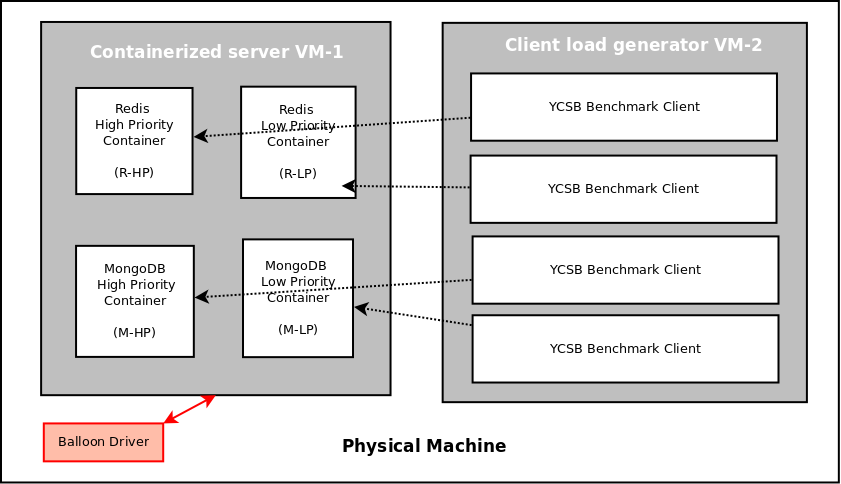
\includegraphics[width=1\textwidth]{images/controller_issues/derivative_setup.png}
	\caption{Derivative cloud testbed}
	\label{img:derived_setup}
      \end{figure}
      
      \paragraph{Host}	
	\begin{enumerate}
	  \item Intel Xeon E5507 @ 2.27GHz
	  \item 8 cores of CPU (with hyper-threading support)
	  \item 125 GB of attached storage, Unlimited NFS attached storage 
	  \item 24 GB RAM
	  \item Ubuntu 14.04 LTS server, 64 bit 
	  \item Kernel version 3.13
	  \item KVM Hypervisor with memory ballooning enabled
	  \item Guest machines were connected using a software bridge
	\end{enumerate}
      
      \myparagraph{Guest}
	The two VMs used in this setup are described here.
	
	\noindent \textbf{VM-1:} Running server containers
	\begin{enumerate}
	  \item 6 cores of pinned CPUs (with hyper threading support)
	  \item 175 GB of virtual disk space (Storage was provisioned using NFS)
	  \item 16 GB RAM
	  \item Ubuntu 16.04 LTS desktop, 64 bit
	  \item Kernel version 4.7
	  \item Container technology: Docker
	  \item Containers inside guest were multiplexed using NAT forwarding
	\end{enumerate}
	
	\noindent \textbf{VM-2:} Running clients that connect to server containers
	\begin{enumerate}
	  \item 1 core of pinned CPU (with hyper threading support)
	  \item 20 GB of virtual disk space (Storage was provisioned using NFS)
	  \item 6 GB RAM
	  \item Ubuntu 16.04 LTS desktop, 64 bit
	  \item Kernel version 4.7
	\end{enumerate}
	
	Redis and MongoDB was used to generate the memory pressure inside the containers. External pressure was generated by varying guest 
balloon size triggered from the host.

      
    \subsubsection{Experimental Flow}
      
      To establish the limitations of nesting-agnostic memory reclamation we performed
      the following experiments. Two Linux+KVM virtual machines were used, one in a nesting setup,
      which hosted containers, the second generated workloads for the 
      container-hosted applications. The nested VM was provisioning with 6 vCPUs
      and 16 GB memory and the workload generating VM has allocated 1 vcPU and 6 GB memory.
      The nesting setup consisted of four Docker containers~\cite{docker}
      which executed with \redis{}~\cite{redis} and
      \mongo{}~\cite{Mongodb} workloads. 
      Default configurations of the applications executed within
      the contains is as shown in Table~\ref{tbl:table_default_config}.
      %The four containers consisted of 2 containers running Redis \cite{redis} and MongoDB \cite{mongodb} workloads each. 
      The YSCB~\cite{cooper2010benchmarking} workbench was used to generate workload datasets and 
      as a workload generator. For the first 100 seconds the applications were executed without 
      memory pressure to consume as much memory as required. Beyond 100 seconds, memory pressure
      was generated from the host and memory from the nested VM reclaimed at rate of 2 GB
      every 30 seconds.

      \begin{table}[t]
	  \begin{center}	   
	    \begin{tabular}{| l | c | c | c | c |}
	      \hline
	      Container & \hl{} (GB) & \sol{} (GB) & \# of records & Usage (GB)  \\ 
	      \hline
	      \hline
	      Redis-Low & 2 & 0.5 & 500K & 1.3 \\  
	      \hline
	      Redis-High & 4 & 1 & 1000K & 2.6 \\  
	      \hline
	      Mongo-Low & 2 & 0.5 & 500K & 1.3 \\
	      \hline
	      Mongo-High & 4 & 1 & 1000K & 2.6 \\
	      \hline
	    \end{tabular}	  
	  \end{center}
	  \caption{Default configuration of the four application containers running in the derivative cloud setup}
	  \label{tbl:table_default_config}	  
	\end{table}
    
     \subsubsection{Impact in derivative environment}
     \label{sec:drawback_env}
	
      \begin{figure*}
	      \begin{subfigure}{0.48\textwidth}
      %	  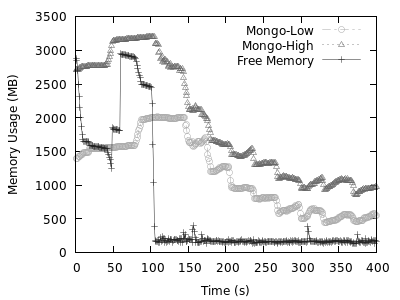
\includegraphics[scale=0.44]{images/inference/memory_usage_mongo.png}
		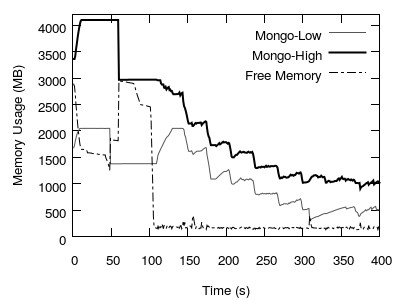
\includegraphics[width=\textwidth]{images/controller_issues/derivative_issues/memory_usage_redis.png}
		\caption{\footnotesize Memory usage for \redis{} applications.}
		\label{plot_inference_redis}
	      \end{subfigure}
	      \begin{subfigure}{0.48\textwidth}
		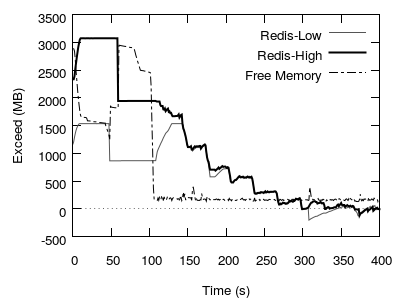
\includegraphics[width=\textwidth]{images/controller_issues/derivative_issues/exceed_redis.png}
		\caption{\footnotesize Extent of memory usage exceed for \redis{} applications.}
		\label{plot_exceed_redis}
	      \end{subfigure}
	    \begin{subfigure}{0.48\textwidth}
      %	  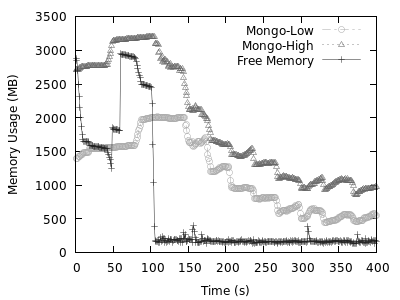
\includegraphics[scale=0.44]{images/inference/memory_usage_mongo.png}
		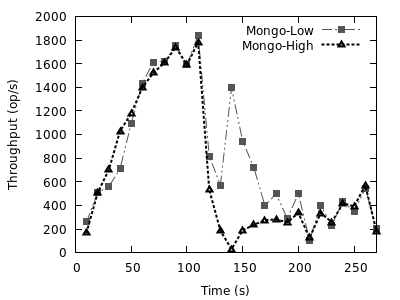
\includegraphics[width=\textwidth]{images/controller_issues/derivative_issues/mongo_throughput.png}
		\caption{\footnotesize Impact of improper memory allocations on \mongo{} applications.}
		\label{plot_throughput_mongo}
	      \end{subfigure}
	      \begin{subfigure}{0.48\textwidth}
		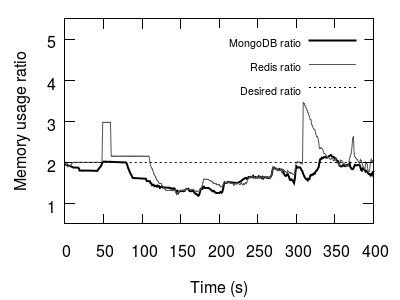
\includegraphics[width=\textwidth]{images/controller_issues/derivative_issues/memory_ratio.png}
		\caption{\footnotesize Memory allocation ratios.}
		\label{plot_inference_ratio}
	      \end{subfigure}
      \caption{Plots illustrating limitations in maintaining memory ratios in derivative clouds}
      \end{figure*}
      
      Figure~\ref{plot_inference_redis} shows the memory consumed by the 
      containers executing the two \redis{} workloads and free memory 
      available in the virtual machine.
      The two containers are configured to consume memory in the ratio of 1:2
      (refer to Table~\ref{tbl:table_default_config}), via \hl{} and \sol{}
      specifications. At 50 seconds, both the \redis{} workloads, which
      are already at their \hl{}, try to allocate more memory, this results
      in container-specific memory reclamation---the free memory in the
      system increases and the memory usage of the two containers drops
      to 1.35 GB and 2.7 GB.
      At 100 seconds, the hypervisor-based balloon controllers starting
      exerting memory pressure---demanding 2 GB every 30 seconds.
      As shown in Figure~\ref{plot_inference_redis}.
      just after 100 seconds, the free memory in the system drastically drops.
      The extent of memory \emph{exceed} beyond 
      the \sol{} specifications is shown in Figure~\ref{plot_exceed_redis}.
      Since, the \redis-high application exceeds by a large extent (2 GB more
      that \sol), the cg{} subsystem penalizes this container for 
      reclamation.
      Further, due
      to the free memory available, and reduced memory consumption of the 
      \redis-high workload, the usage for the \redis-low application 
      increases for an epoch and just before 150 seconds, the extent
      of exceed beyond the \sol{} specifications for both the containers
      is similar. \emph{Note that this is how the cg{} subsystem operates,
      it penalizes the container with the maximum extent of exceed, till
      all of them exceed by the same absolute value and then 
      penalizes them equally.} This process essentially does not
      adhere to the memory usage ratios that were expected with the
      \sol{} and \hl{} specifications. Figure~\ref{plot_inference_ratio}
      shows the memory usage of the \redis{} and \mongo{} applications,
      which drops below the 1:2 ratio from 100 seconds to 300 seconds.
      At 300 seconds, the extent of exceed decreases to zero and
      the system switches to the global reclamation (GLR) mode.
      Beyond this point, the memory reclaimed is not container-agnostic
      and variable ratios of usages are observed.
    
    \subsection{Key Implications}
    The key takeaways from these experiment are as follows,
      \begin{itemize}
      \item Memory reclamation uses the extent of exceeded usage above a containers \sol{}.
      Containers with higher exceed values are penalized to a larger extent.
      \item The Linux cg{} systems attempts to maintain similar extent of exceed for
      memory usage during reclamation when all container are above their \sol's.
      %Reclamation is based on exceed values of each container when any of the containers are using more memory than their SLs. Containers with higher exceed values will be penalized more. Reclamation falls back to host LRU based reclamation without considering container provisioning when memory usage of every containers are below their SLs. Can user provide/ensure priority to a container over other containers using existing memory control knobs (SL and HL)?
      % \item Reclamation falls back to host LRU based reclamation without considering container provisioning when memory usage of every containers are below their SLs. %Priority definition on the basis of SL and HL will become useless if exceed of all containers are zero.
      % Can we define priority of containers using SL and HL?
      \item A per-container \sol{} and \hl{} specification does not guarantee proportionate
      memory allocation during memory pressure situations.
      %Soft Limit is not a definite guarantee, it is mere best effort approach. Can we ensure SL as a definite guarantee to higher priority container(s), if possible?
      \end{itemize}
      This Linux \cg{} reclamation policy does not accommodate different user-specified policies
      that are desired---proportionate memory usages at all instances,
      order-of-reclamation across containers etc. This is especially required in nested
      hosting environments where derivative service provides would be benefited
      by providing a rich set of prioratization features.
    
  \section{Requirements for a new memory management controller}
  
    We wish to build an updated memory management controller that is controller aware, and is able to enforce a differential management
    policy by a native or derivative cloud provider. The following are the list of requirements of policies that we would like to enforce
    using this controller,
  
    \begin{enumerate}
      \item \textbf{Prioritized memory allocation:} Currently the notion of priority doesn't exist in container specific memory allocation 
although the notion of priority exists in other resources. The existing knobs fail to enforce priority used to manage memory in containers. 
      \item \textbf{Deterministic provisioning:} The policy to be designed must eliminate existing non determinism that exists while 
managing memory between containers in existing system.
      \item \textbf{Elastic provisioning:} Memory allocated must be re-sizable as and when required. 
      \item \textbf{Adaptive:} On changing resources provisioned to the system as in the case of an derivative environment, the policy 
enforced must still do it's best in maintaining promised QOS.
      \item \textbf{Differentiated memory reclamation:} The policy could build around the notion of differentiated memory reclamation when 
the system falls under memory pressure.
      \item \textbf{Strict enforcement of limits:} The notion of hard and soft limits that exist must be strengthened.      
    \end{enumerate}
    
  We would like to design a new controller keeping the above requirements in mind.
   
  
  \section{Proposed memory management controller}
      
      Enforcing memory allocation proportions across containers when no memory pressure exists is possible with the soft-limit and hard-limit 
      configuration parameters. However, as discussed in Section~\ref{sec:controller_issues}, these knobs do not provide deterministic memory 
      provisioning when the system is under memory pressure. As part of this work, we design for two new policies to provide deterministic 
      memory provisioning in nested setups under memory pressure
      
      \subsection{Controller logic}
	When the VM in which the containers are executing comes under memory pressure, memory is reclaimed using the container specific LRU lists 
	(as SMR) as well as the Global LRU list (as GLR) by the guest operating system.
	Memory reclamation depends on the extent of \textit{exceed} in memory usage above the specified \sol---estimated as the difference 
	in the two values. 
	The container having a higher \textit{exceed} is victimized during memory pressure first.
	We redefine this notion of \textit{exceed} with one that is based on proportionality weight of each container. 
	The proportional allocation of a container is the ratio of the container weight to the total weight across all containers in a 
	VM multiplied by the total memory usage across all containers (Equation~\ref{eqn:pa}). The proportionate \textit{exceed} value is the 
	difference of the container's proportional memory allocation and its current usage (Equation~\ref{eqn:ex}). 
	Finally, the memory reclamation policy is modified to target the container having  the highest proportionate \textit{exceed} value for each
	reclamation request. Similar to the default reclamation policy, the global LRU list for reclamation is used once memory usage 
	of all containers is below \sol{} specifications.
	
	\small
	\begin{align}
	  T\_U &= \sum_{i=1}^{n}U_{i} \\
	  T\_W &= \sum_{i=1}^{n}W_{i} \\
	  PA_{i} &= T\_U \times (\frac{W_{i}}{T\_W}) \label{eqn:pa}\\
	  EX_{i} &= U_{i} - PA_{i} \label{eqn:ex}
	\end{align}

	\footnotesize
	\textit{
	\\
	U$_{i}$: Memory usage of i$^{th}$ container \\
	W$_{i}$: Relative weight of i$^{th}$ container \\
	T\_U: Total memory usage by all containers \\
	T\_W: Summation of relative weights of all containers \\
	PA$_{i}$: Proportional memory allocation of i$^{th}$  container \\
	EX$_{i}$: Proportionate exceed value of i$^{th}$ container
	}
	\normalsize
    
      \subsection{Policies supported by our controller}
      
	The following are the policies enforceable by our controller.  
	
	\subsubsection{Policy 1: Proportionate memory allocation}
	  This policy aims to ensure that all memory allocated to container is based on relative weights specified as configuration parameters.
	  The proportional memory allocation is enforced during situations of memory pressure and during no pressure. For example, consider 
	  two containers with an intended proportionate memory allocation in the ratio 1:2. Further, assume that their \sol{} values are set 
	  to 1 GB and 2 GB, respectively, and their current usage is 2 GB and 4 GB respectively.
	  With a memory reclamation demand of 1 GB, most of the memory will be reclaimed from the container with the larger extent of usage, 
	  since the extent of exceed is 2 GB as compared to 1 GB of the smaller container. The resulting usages after reclamation will be 2 GB 
	  and 3 GB, respectively, violating the proportionate ratio of 1:2. The proposed proportionate allocation policy aims to maintain 
	  the 1:2 ratio in all memory pressure situations.
	
	\subsubsection{Policy 2: Application-specific differentiated allocation}
	\label{sec:memory_distribution}
	  This policy provides the flexibility of providing specific rules and or categories to application containers, e.g. gold, silver,
	  bronze etc. Containers mapped to each of these categories have different reclamation rules or the categories themselves can 
	  imply an ordering for reclamation.
  
  \section{Modifications made to Linux memory Cgroup}
      
      We modify memory Linux \cg{} memory management subsystem to conform to the polices specified earlier. We have made
      three major changes to this subsystem as described below.
     
    
    \subsection{Per container configurable weights}
      A new per-cgroup state variable is introduced to specify a \emph{weight}
      parameter for each container and is also
      exposed through \texttt{sysfs} interface for every container.
      These weights enforce a notion of priority among containers; 
      higher the weight for a container the higher its priority and proportion.
      The relative ratio of the weights, dictate the proportion of memory allocation.
      Cloud providers can modify these weights in the derivative setup 
      (also applicable to native cloud providers using 
      containers for provisioning) to enforce priority among containers 
      executing within VMs.
    
    \subsection{Flexible reclamation size}
      The current soft-memory reclamation policy (SMR), targets one container and 
      reclaims a non-deterministic amount of memory from it for every 
      request. The extent of reclamation depends on the anonymous region (from which
      a fixed size is reclaimed) and the disk page cache (from which a large
      portion is reclaimed). Since the page cache size is non-deterministic,
      reclamation extent can also be non-deterministic.
      This may lead to a container being targeted exclusively for a particular 
      reclamation request, leading to large deviations 
      from weighted allocations. To overcome this issue, we have 
      capped reclamation chunk size to a maximum of 50 MB. 
    
    \subsection{Deterministic reclamation}
      As part of the Linux \cg{} memory reclamation process, soft-reclamation (SMR)
      reclaims memory from each container till memory usage is above the
      \sol specification. Simultaneously, a small amount of memory is also
      reclaimed from the system-wide pool of pages (GLR). In our solution,
      to maximize deterministic reclamation we perform proportionate
      reclamation across containers till the usage of containers reduces
      to zero. Beyond this situation, the system-wide global LRU list is
      used for further reclamations.
      Since the SMR policy is container-aware, this strategy
      provides us a better handle over memory provisioning for containers. 
    
  
  \section{Empirical evaluation of our controller}
       
    We show the effectiveness of our approach empirically in this section. Experimental set-up for the most part remains same as that 
mentioned in Section~\ref{sec:derivative_testbed}. Any changes to the set-up is mentioned in the respective subsections.

    Experiments are performed with the same workload and set-up except for the size of VM-1. At the beginning of the experiment, size of VM-1 
is 20 GB which is gradually reduced to 3.5 GB, at the rate of 1.5 GB every 20s (started at 50s). Relative memory weights for the \mongo{} 
containers are in the ratio of 1:2 (1 for low and 2 for high priority containers) as are the relative weights for the \redis{} 
containers. These weights are added using the newly added \textit{weight} parameter in the memory \textit{Cgroup}. 

% \begin{figure}
% 	  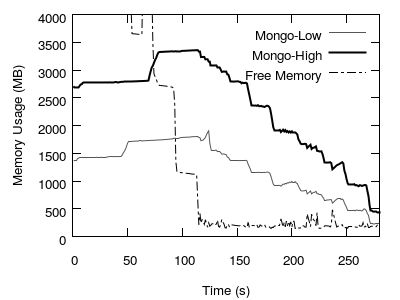
\includegraphics[scale=0.45]{images/mem_sol/sl=hl_mtp/memory_usage.png}
% 	  \caption{\footnotesize Memory usage by Mongodb containers when SL=HL, using modified controller}
% 	  \label{mem_sol_sl=hl_mongo}
% \end{figure}
% 	~
% \begin{figure}
% 	  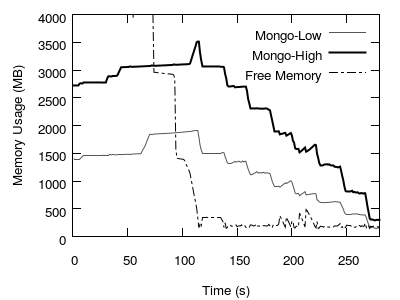
\includegraphics[scale=0.45]{images/mem_sol/sl!=hl_mtp/memory_usage.png}
% 	  \caption{\footnotesize Memory usage by Mongodb containers when SL!=HL, using modified controller}
% 	  \label{mem_sol_sl!=hl_mongo}
% \end{figure}	
	

\begin{figure*}
	\begin{subfigure}{0.30\textwidth}
	  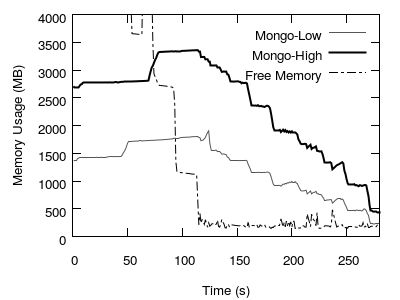
\includegraphics[scale=0.4]{images/mem_sol/sl=hl_mtp/memory_usage.png}
	  \caption{\footnotesize Memory usage by Mongodb containers when SL=HL}
	  \label{mem_sol_sl=hl_mongo}
	\end{subfigure}
	~
	\begin{subfigure}{0.30\textwidth}
	  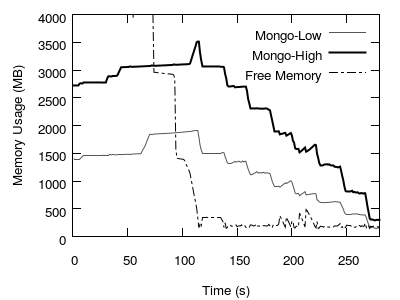
\includegraphics[scale=0.4]{images/mem_sol/sl!=hl_mtp/memory_usage.png}
	  \caption{\footnotesize Memory usage by Mongodb containers when SL$\neq$HL}
	  \label{mem_sol_sl!=hl_mongo}
	\end{subfigure}	
	~
	\begin{subfigure}{0.30\textwidth}
	  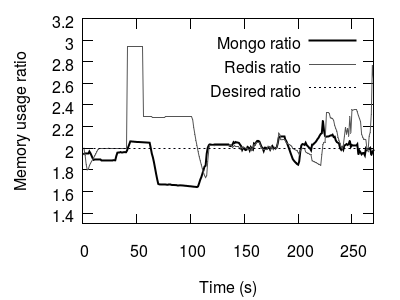
\includegraphics[scale=0.4]{images/mem_sol/memory_ratio_base.png}
	  \caption{\footnotesize Memory usage ratios between MongoDB and Redis containers}
	  \label{mem_sol_ratios}
	\end{subfigure}
	~
	\begin{subfigure}{0.5\textwidth}
	  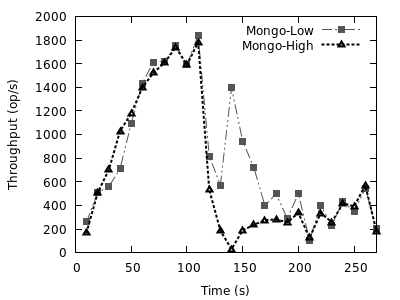
\includegraphics[scale=0.6]{images/mem_sol/mongo_before.png}
	  \caption{\footnotesize Application throughputs with existing memory controller}
	  \label{throughput_mongo_before}
	\end{subfigure}
	~
	\begin{subfigure}{0.5\textwidth}
	  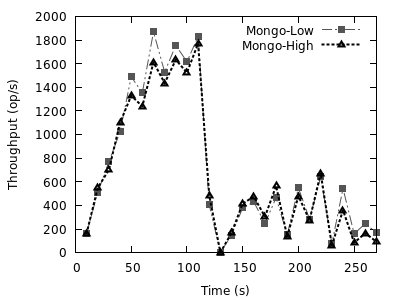
\includegraphics[scale=0.6]{images/mem_sol/mongo_after.png}
	  \caption{\footnotesize Application throughputs with modified memory controller}
	  \label{throughput_mongo_after}
	\end{subfigure}	
  \label{fig:mem_sol}
\caption{Impact of modified controller on low and high priority containers}
\end{figure*}

  
    \subsection{Effectiveness of our controller}
    
      We have tested the effectiveness of our approach in both cases: (i) Soft Limit is equal to Hard Limit (SL=HL) and (ii) Soft Limit is not 
equal to Hard  Limit (SL$\neq$HL), because memory reclamation methods for both cases are different as mentioned in Section~\ref{sec:mem_management}. 

Figure \ref{mem_sol_sl=hl_mongo} and Figure \ref{mem_sol_sl!=hl_mongo} depicts the memory usage patterns for \mongodb{} containers for cases 
(i) and (ii) respectively. We observe a gradual decrease in memory allocated to the low and high priority containers in both cases once the 
system runs out of free memory at about 120 seconds. The ratios of memory allocated to containers can be seen to be in accordance with
their relative weights, unlike the earlier case when there is no modified controller.
We observed similar pattern in case of \redis{} container. 
%However unlike the earlier case (without our modified controller), the memory allocated to containers are in the ratios according to their relative weights. Similar pattern is also observed for Redis containers. 
This pattern of relative memory allocations can be observed more prominently when comparing Figure \ref{plot_inference_ratio} and Figure \ref{mem_sol_ratios} 
which shows memory usage ratios between low and high priority containers (closer to 2, the better) using existing controller and our 
modified controller respectively.

The effect of better memory allocation is notable in the application throughputs. The existing controller produces better throughputs 
for the lower priority \mongodb{} containers in the interval 100-200s as seen in Figure \ref{throughput_mongo_before}. With our modified 
controller, both the low priority and high priority containers produce similar throughput as seen in Figure \ref{throughput_mongo_after}. 
The similar throughputs observed are strongly connected to the fact that low and high priority containers are provisioned with 1:2 memory 
allocations and so are the ratio between their usage patterns (Provisioning is done to avoid contention due to any other resource). Similar 
throughput impacts are also observed with \redis{} containers. Hence credit share not only produces better memory allocations, but also 
enhances application performance for containers.
    
    \subsection{Differential QOS containers}
    
      Consider the application specific differentiated allocation policy specified in Section 
\ref{sec:memory_distribution} where we would like to prioritize a container from being 
victimized. Let's call this container as a gold container. We have used same set-up 
(SL$\neq$HL) to test this. We have prioritized the gold container using the higher weights 
(Weights of the order of $10^{3}$ relatively higher) to avoid reclamation from it unless it's necessary.
There are also other containers running inside the VM with lower QOS and let's call them silver containers.

In Figure \ref{priority_cont} we have plotted only the memory usage for the gold and one silver container for ease of analysis. We 
observe that at about 120 seconds free memory drops and the reclamation kicks in. Victimization of gold container is much lesser than other 
containers until the other containers usage near zero. This shows how we could use our weighted controller to enforce differential 
service QOS containers.

\begin{figure}
  \centering
  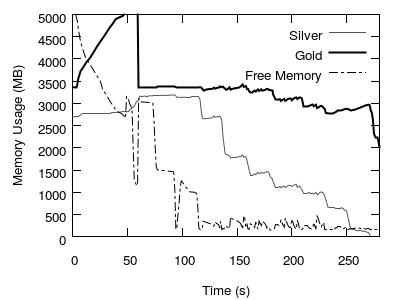
\includegraphics[scale=0.6]{images/mem_sol/gold/memory_usage.png}
  \caption{Memory usage plot showing implication of relative weights provide differential QOS guarantees}
  \label{priority_cont}
\end{figure}
    
    \subsection{Impact of reclamation chunk size}
    
    
    The native reclamation method has no notion of limit on the
amount of memory that can be reclaimed from a targeted container. This leads to larger 
reclamation amounts from a container thereby deviating it from the desired relative 
allocations.

Figure \ref{mem_ratio} shows the ratio of memory usage between \mongodb{} containers for default (native) case and reclamation
chunk size of 50 MB. We consider observation after 120 seconds, as that is when the pressure kicks in and triggers 
reclamation. Although the 50 MB capping of reclamation chunk provides better memory ratios than the default case most of
the time, it still deviates from desired behavior in the interval 180-220 seconds as seen in Figure~\ref{mem_ratio}. 

With smaller maximum reclamation size, we will have finer control over the memory allocation ratios, but this 
comes at the cost of frequent updation. Further investigation has to be done to fix upon a reasonable size to 
maintain balance between performance and precision here. For now, the reclamation chunk size is parameterized in our implementation and can 
be easily modified using a kernel module to alter the maximum reclamation chunk size. We have used reclamation chunk size of 50 MB in our 
implementation and this applies to all the experiments that we have run with our modified controller.

\begin{figure}
  \centering
  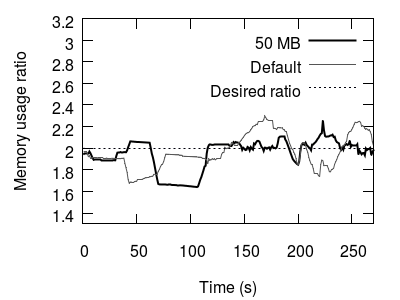
\includegraphics[scale=0.6]{images/mem_sol/memory_ratio.png}
  \caption{Memory usage ratio with different reclamation chunk size}
  \label{mem_ratio}
\end{figure}